\section{Clasificación: Análisis Estadístico de Datos}

\subsection{Introducción}

Para el problema de clasificación hacemos uso del dataset \textbf{haberman} \cite{haberman}, que codifica el ratio de supervivencia de pacientes operados de cáncer de pecho en el Hospital Universitario de Chicago, en base a las siguientes características:

\begin{enumerate}
\def\labelenumi{\arabic{enumi}.}
    \item \textbf{Age}: Indica la edad del paciente en el momento de la operación.
    \item \textbf{Year}: Los dos últimas cifras del año en el que se operó el paciente.
    \item \textbf{Positive}: Número de nodos auxiliares positivos detectados. Esta variable hace referencia a los ganglios linfáticos que dan positivos como presentes de cáncer. A mayor número de nodos detectados, mayor es la gravedad del cáncer. 
    
    Aunque normalmente la primera zona de propagación del cáncer son estos nodos, no es la única medida de la seriedad, pues este puede propagarse a otras zonas del cuerpo. En principio no deberíamos descartar la posibilidad de que puede haber casos de no supervivencia con bajo número de positivos.

    Viendo que solo tenemos esta medida del cáncer en el dataset es posible que la operación que recibieron los pacientes sea algún tipo de cirugía de ganglios linfáticos, donde el cirujano intenta extraer los nodos afectados por el tumor. Por consiguiente, cuanto mayor es la cantidad de nodos detectados, más complicaciones pueden acarrearse de la operación \cite{cancer1, cancer2}.
\end{enumerate}

El objetivo es poder clasificar, en base a los tres atributos, si los pacientes pueden sobrevivir 5 años o más:

\begin{enumerate}
    \def\labelenumi{\arabic{enumi}.}
    \setcounter{enumi}{3}
    \item \textbf{Survival}: Sí/No indicando la supervivencia del paciente tras 5 años.
\end{enumerate}

Contamos por tanto con un problema de clasificación binario en base a tres características, y con un número total de 306 instancias.

\vspace{\baselineskip}

La descripción del problema nos da alguna información adicional sobre las variables:

\begin{enumerate}
    \def\labelenumi{\arabic{enumi}.}
    \item \textbf{Age}: Variable numérica discreta, contamos con valores enteros en el
    rango {[}30,83{]}.
    \item \textbf{Year}: Variable numérica discreta, contamos con valores enteros en el
    rango {[}58,69{]}.
    \item \textbf{Positive}: Variable numérica discreta, contamos con valores enteros en
    el rango {[}0,52{]}.
    \item \textbf{Survival}: Variable binaria.
\end{enumerate}

\paragraph{Hipótesis de partida}

\begin{itemize}
    \item \textbf{H.1}: Habrá menor ratio de supervivencia cuanto mayor sea el número de nodos positivos encontrados.
    \item \textbf{H.2}: Habrá mayor ratio de supervivencia cuanto más joven sea el paciente.
    \item \textbf{H.3}: El rango de Year es pequeño. La influencia de esta variable creemos que podría darse solo si durante ese período se hubieran descubierto técnicas mejores de cirugía. Este razonamiento va orientado de cara a la población y no a la muestra. Puesto que contamos con datos de un solo hospital durante pocos años, es posible que el equipo de cirugía hubiera sido el mismo para la mayoría de pacientes.
    \item \textbf{H.4}: Podría haber relación entre la edad y el número de positivos, posiblemente indicando lo tardío que se descubre el cáncer.
    \item \textbf{H.5}: La bibliografía nos dice que el cáncer puede aparecer a diferentes edades con diferentes factores de riesgo (alcoholismo, herencia genética\ldots). Podría ser que el número de variables con las que contamos sea insuficiente para la clasificación. (Hipótesis no demostrable en el EDA).
\end{itemize}

\subsection{Análisis Estadístico de Datos}

R por defecto nos carga las variables Age, Year y Positive como numéricas y Survival como carácter.
Transformamos Survival a factor categórico, el resto de variables las mantenemos en su formato.

\subsubsection{Análisis univariable}

La cabecera de los datos nos quedan por tanto de la siguiente manera:
\vspace{\baselineskip}

\begin{tabular}{r|r|r|l}
    \hline
    Age & Year & Positive & Survival\\
    \hline
    38 & 59 & 2 & No\\
    \hline
    39 & 63 & 4 & No\\
    \hline
    49 & 62 & 1 & No\\
    \hline
    53 & 60 & 2 & No\\
    \hline
    47 & 68 & 4 & No\\
    \hline
    56 & 67 & 0 & No\\
    \hline
\end{tabular}

\vspace{\baselineskip}

Con las siguientes medidas estadísticas principales:

\begin{verbatim}
      Age             Year          Positive      Survival 
 Min.   :30.00   Min.   :58.00   Min.   : 0.000   No :225  
 1st Qu.:44.00   1st Qu.:60.00   1st Qu.: 0.000   Yes: 81  
 Median :52.00   Median :63.00   Median : 1.000            
 Mean   :52.46   Mean   :62.85   Mean   : 4.026            
 3rd Qu.:60.75   3rd Qu.:65.75   3rd Qu.: 4.000            
 Max.   :83.00   Max.   :69.00   Max.   :52.000            
\end{verbatim}

En las distribuciones de los clasificadores nos fijaremos más adelante. Aquí hacemos notar que los valores de salida en nuestros datos están bastante desbalanceados, solo un 26.5\% de los paciente sobrevivieron a los 5 años.

\newpage

El dataset cuenta con valores 17 repetidos, concretamente las siguientes ocurrencias:
\vspace{\baselineskip}

\begin{tabular}{r|r|r|l}
\hline
Age & Year & Positive & Survival\\
\hline
37 & 63 & 0 & No\\
\hline
37 & 63 & 0 & No\\
\hline
38 & 60 & 0 & No\\
\hline
38 & 60 & 0 & No\\
\hline
41 & 65 & 0 & No\\
\hline
41 & 65 & 0 & No\\
\hline
43 & 64 & 0 & Yes\\
\hline
43 & 64 & 0 & Yes\\
\hline
44 & 61 & 0 & No\\
\hline
44 & 61 & 0 & No\\
\hline
48 & 58 & 11 & Yes\\
\hline
48 & 58 & 11 & Yes\\
\hline
50 & 61 & 0 & No\\
\hline
50 & 61 & 0 & No\\
\hline
54 & 62 & 0 & No\\
\hline
54 & 62 & 0 & No\\
\hline
& & &\\
\hline
\end{tabular}
\begin{tabular}{r|r|r|l}
\hline
Age & Year & Positive & Survival\\
\hline
55 & 58 & 1 & No\\
\hline
55 & 58 & 1 & No\\
\hline
56 & 60 & 0 & No\\
\hline
56 & 60 & 0 & No\\
\hline
57 & 64 & 0 & No\\
\hline
57 & 64 & 0 & No\\
\hline
61 & 59 & 0 & No\\
\hline
61 & 59 & 0 & No\\
\hline
61 & 59 & 0 & No\\
\hline
62 & 66 & 0 & No\\
\hline
62 & 66 & 0 & No\\
\hline
63 & 63 & 0 & No\\
\hline
63 & 63 & 0 & No\\
\hline
65 & 64 & 0 & No\\
\hline
65 & 64 & 0 & No\\
\hline
67 & 66 & 0 & No\\
\hline
67 & 66 & 0 & No\\
\hline
\end{tabular}

\vspace{\baselineskip}

Existen dos posibilidades para el origen de estos datos:

\begin{enumerate}
    \def\labelenumi{\arabic{enumi}.}
    \item Errores en la introducción de los datos. Entradas repetidas por error.
    \item Son entradas de pacientes distintos casualmente con las mismas características.
\end{enumerate}

Apreciamos que en la mayoría de instancias el número de Positive es cero. En el apartado 3.3 se explica como este es un valor bastante frecuente en los datos pero que posiblemente se deba a que es una medida de los nodos \textbf{auxiliares} y no un error de codificación.

\vspace{\baselineskip}

Como en este caso tenemos muy pocas variables (y un número moderado de entradas, 306), es probable que los pacientes coincidan en las características. Además, podemos ver que las entradas en la mayoría de los casos solo están duplicadas (solo hay una entrada triplicada).

\vspace{\baselineskip}

Por tanto proseguimos sin eliminar estas instancias duplicadas.

\newpage
Mostramos scatterplots univariables:
% \begin{figure}[H]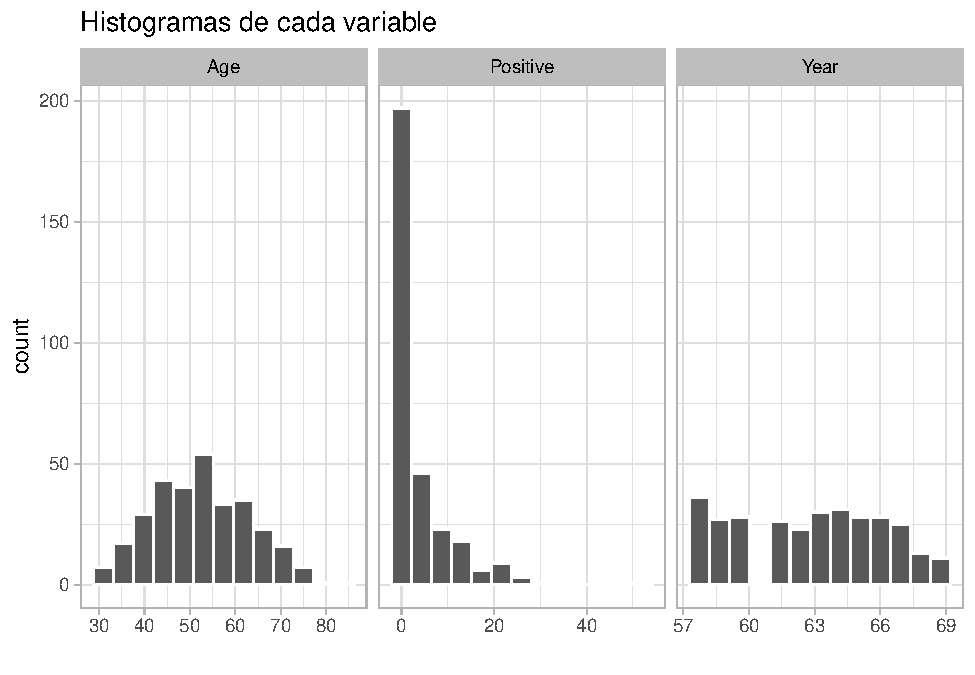
\includegraphics[width=.9\linewidth]{img/EDA2_files/figure-latex/unnamed-chunk-9-1} \caption{}\end{figure}

\begin{figure}[H]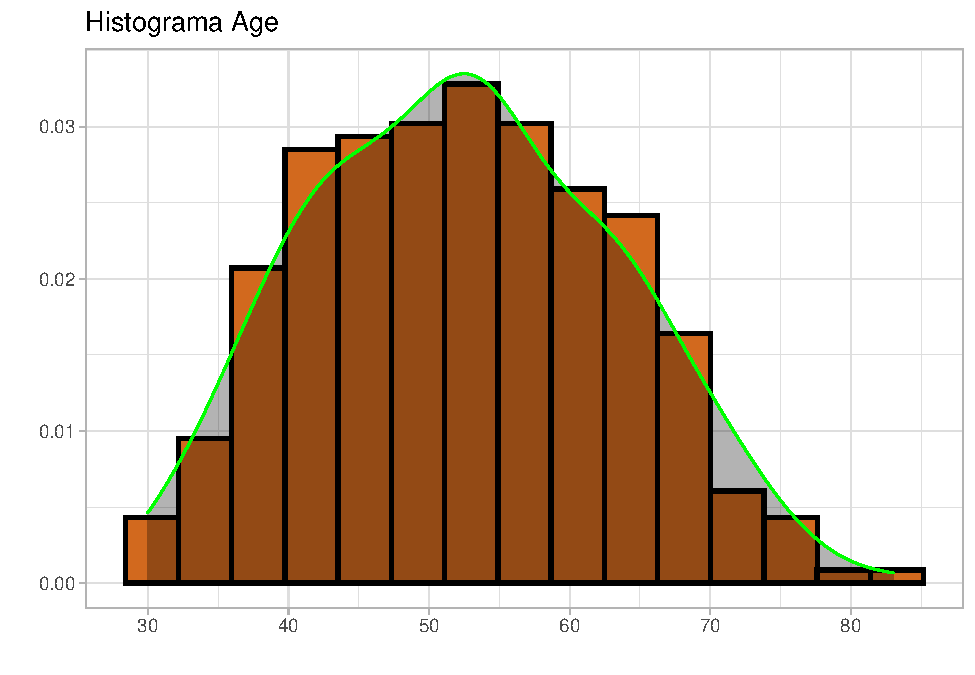
\includegraphics[width=.9\linewidth]{img/EDA2_files/figure-latex/unnamed-chunk-10-1} \caption{}\end{figure}

\begin{figure}[H]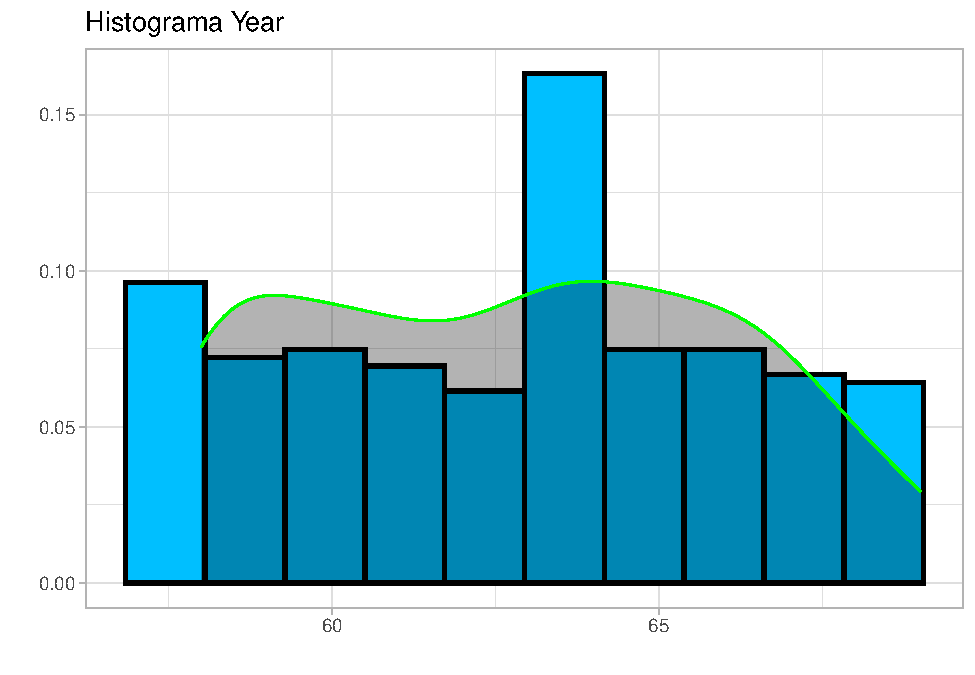
\includegraphics[width=.9\linewidth]{img/EDA2_files/figure-latex/unnamed-chunk-10-2} \caption{}\end{figure}

\begin{figure}[H]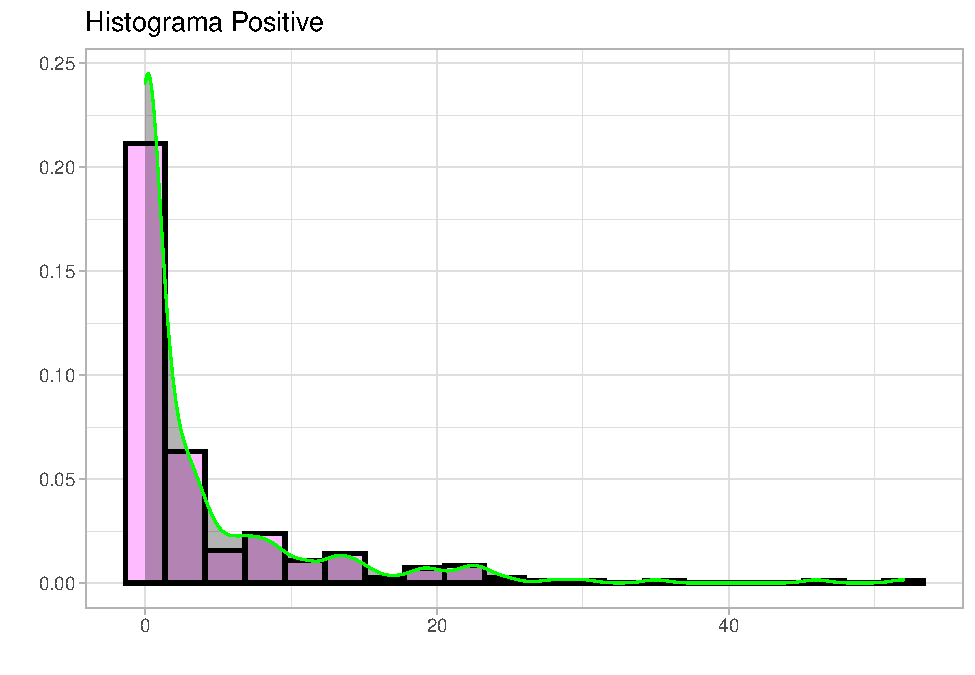
\includegraphics[width=.9\linewidth]{img/EDA2_files/figure-latex/unnamed-chunk-10-3} \caption{}\end{figure}

\begin{figure}[H]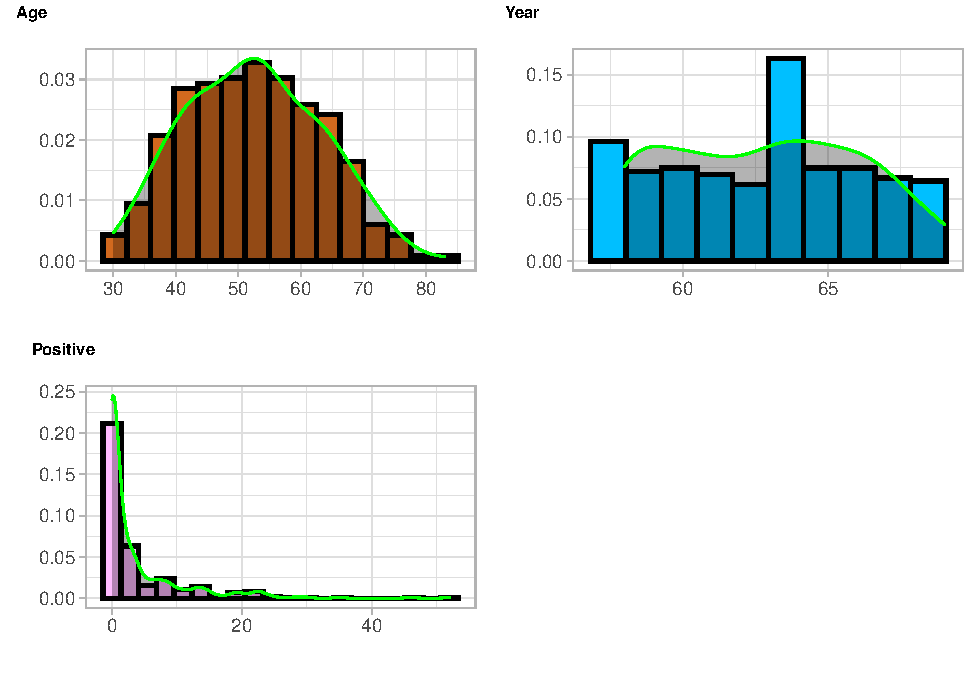
\includegraphics[width=.9\linewidth]{img/EDA2_files/figure-latex/unnamed-chunk-10-4} \caption{}\end{figure}

\newpage

Y boxplots sobre las distribuciones de los datos:
\begin{figure}[H]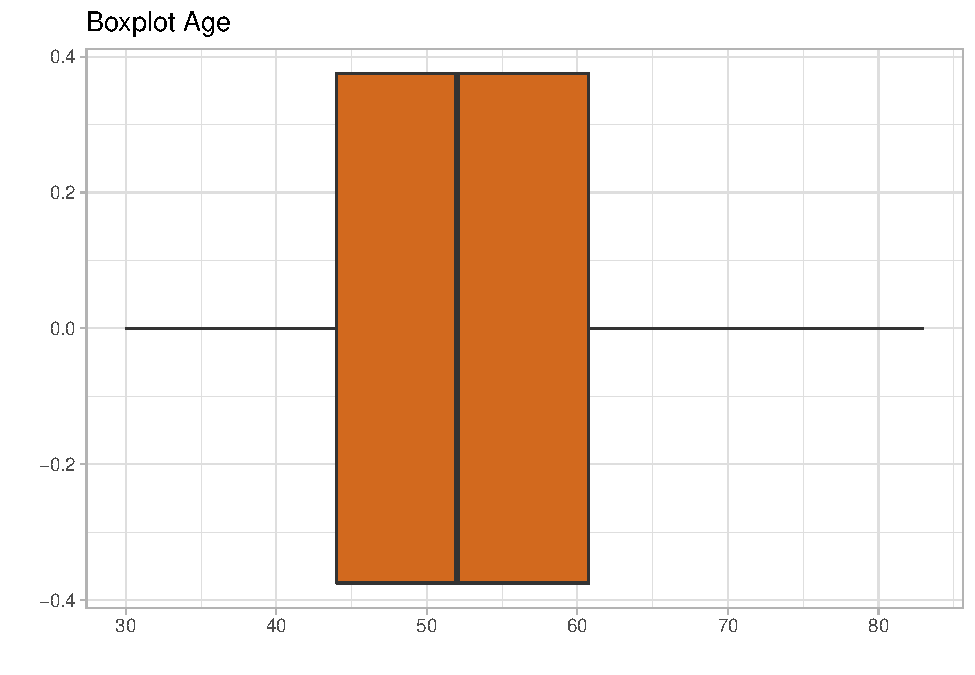
\includegraphics[width=.9\linewidth]{img/EDA2_files/figure-latex/unnamed-chunk-11-1} \caption{}\end{figure}

\begin{figure}[H]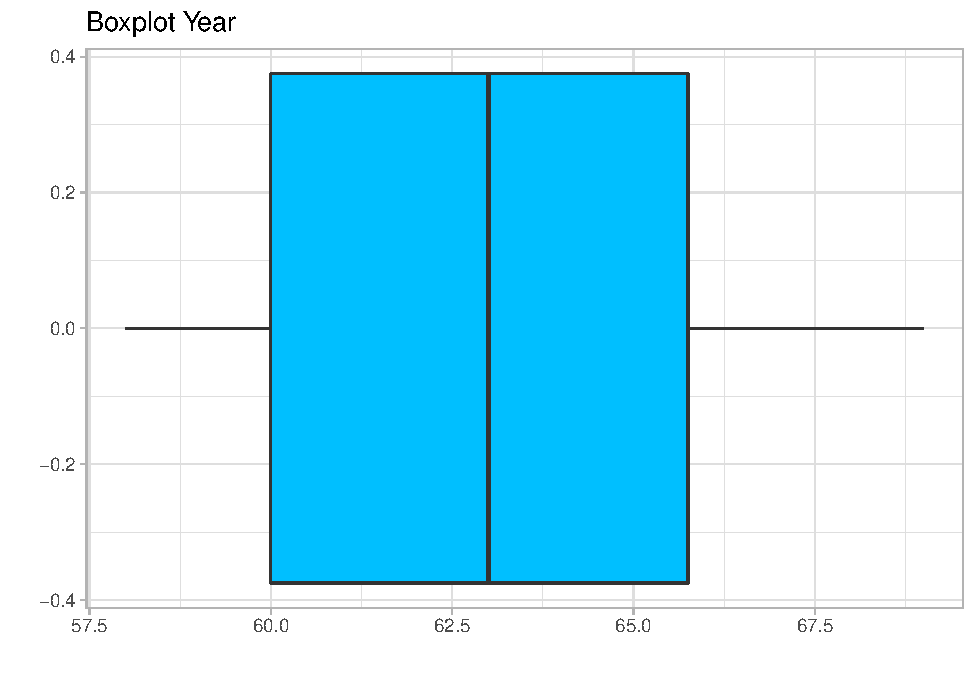
\includegraphics[width=.9\linewidth]{img/EDA2_files/figure-latex/unnamed-chunk-11-2} \caption{}\end{figure}

\begin{figure}[H]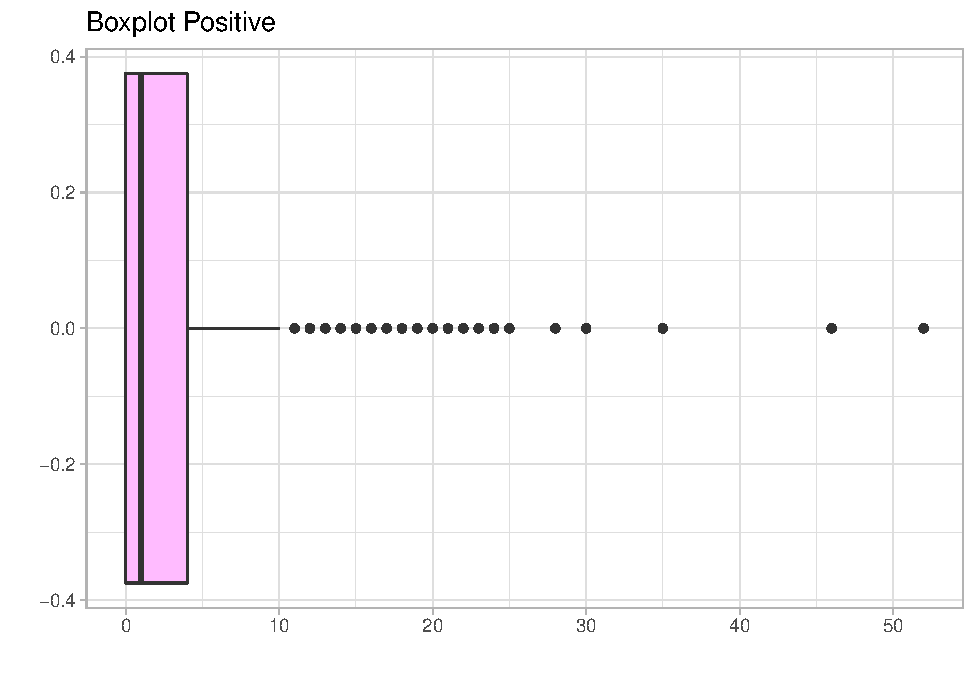
\includegraphics[width=.9\linewidth]{img/EDA2_files/figure-latex/unnamed-chunk-11-3} \caption{}\end{figure}

\begin{figure}[H]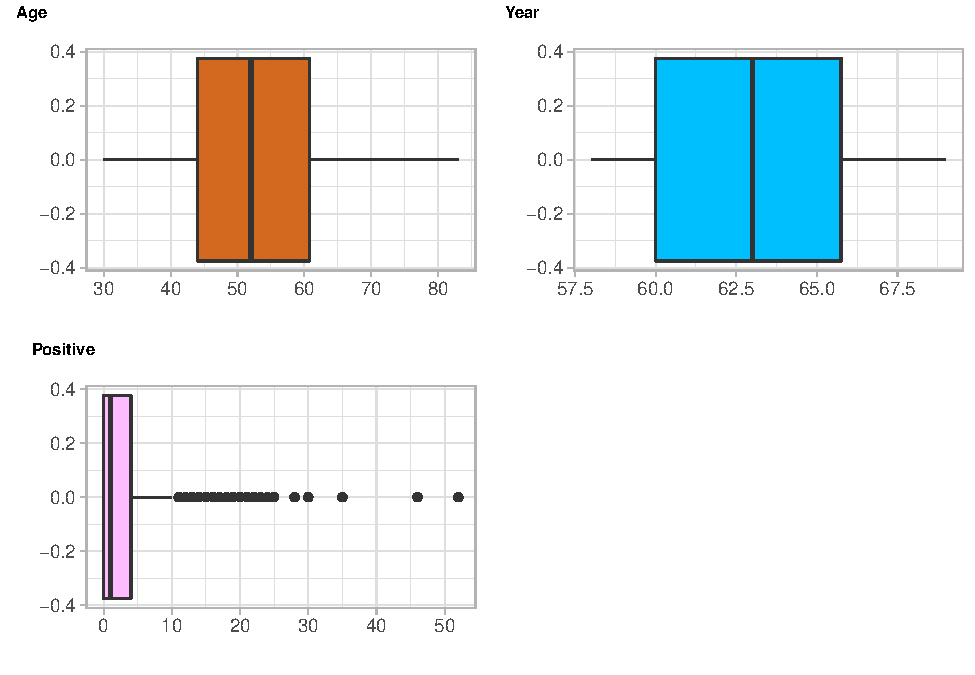
\includegraphics[width=.9\linewidth]{img/EDA2_files/figure-latex/unnamed-chunk-11-4} \caption{}\end{figure}

\begin{figure}[H]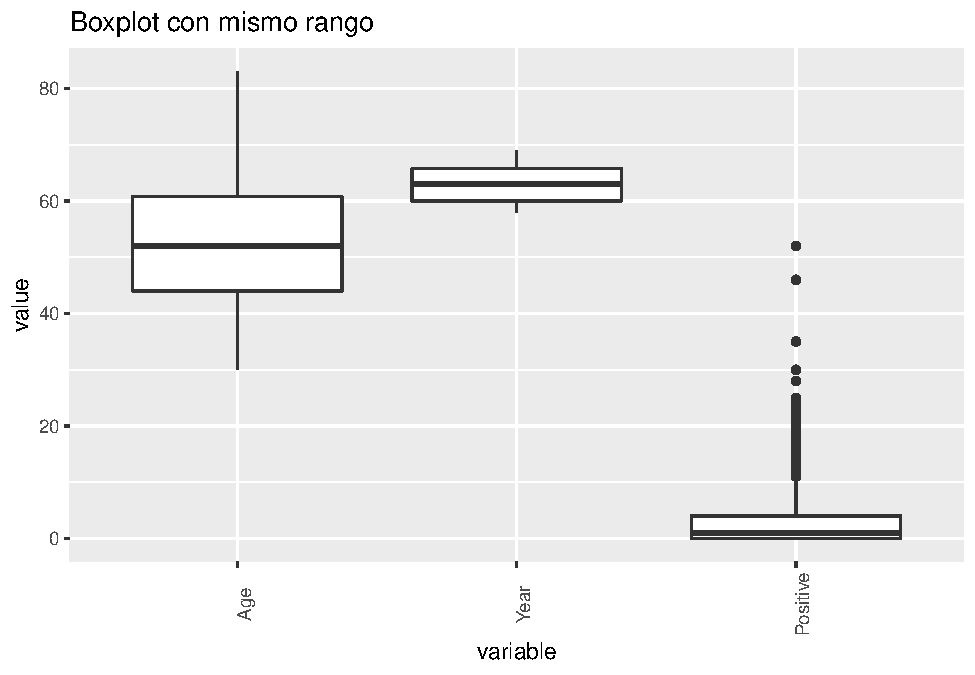
\includegraphics[width=.9\linewidth]{img/EDA2_files/figure-latex/unnamed-chunk-12-1} \caption{}\end{figure}

\vspace{\baselineskip}

Podemos comparar los rangos intercuartiles si estandarizamos antes el dataset
\begin{verbatim}
     Age     Year Positive 
1.550430 1.769555 0.556355 
\end{verbatim}

También podemos ver la distancia entre mínimos y máximos

\begin{verbatim}
     Age     Year Positive 
4.905839 3.385235 7.232616 
\end{verbatim}

Ya la descripción del problema nos lo decía, los rangos en los que se distribuyen los datos son muy diferentes entre sí. Es necesario aplicar un proceso de estandarización antes de clasificar.

\subsubsection{Missing values}

Nos cuestionamos la ocurrencia de instancias con cero en el número de positivos. Podríamos pensar que se trata de una codificación de missing values si nos aseguramos que la operación consistía en eliminar estos nodos positivos.

\vspace{\baselineskip}

Si revisamos la información que tenemos, estos nodos positivos se denominan auxiliares, y una mayor investigación del problema por internet nos asegura de que estos valores de cero no se corresponden a missing values.

Pese a ello, lo apropiado habría sido ponerse en contacto con los creadores del dataset y preguntar por la forma de codificar los datos que habían usado.

\vspace{\baselineskip}

Si hubiéramos descubierto que sí lo son, y tras ver que una gran parte de las instancias contienen este valor, habríamos tenido que buscar algún tipo de imputación para rellenar estos valores. Puesto que tendríamos un número pequeño de valores reales, probablemente habríamos optado por KNN o interpolación lineal.

\paragraph{Age}
Para esta variable no contamos con valores de todos los años, y hemos visto que en general no están equitativamente distribuidos:

\begin{verbatim}
Años:   30 31 33 34 35 36 37 38 39 40 41 42 43 44 45 46 47 48 49 50 51 52
Conteo:  3  2  2  7  2  2  6 10  6  3 10  9 11  7  9  7 11  7 10 12  6 14
Años:   53 54 55 56 57 58 59 60 61 62 63 64 65 66 67 68 69 70 71 72 73 74
Conteo: 11 13 10  7 11  7  8  6  9  7  8  5 10  5  6  2  4  7  1  4  2  2
Años:   75 76 77 78 83
Conteo:  1  1  1  1  1
\end{verbatim}

\paragraph{Year}
Aquí si contamos con valores en todos los años, aunque con más instancias en los iniciales:

\begin{verbatim}
Años:   58 59 60 61 62 63 64 65 66 67 68 69 
Conteo: 36 27 28 26 23 30 31 28 28 25 13 11 
\end{verbatim}


\paragraph{Positive}
Esta variable parece llevar una distribución exponencial y probablemente por ello aparezcan tantas posibles anomalías.

\subsubsection{Análisis sobre las distribuciones}

Ninguna variable parece seguir una distribución semejante a una distribución normal. Lo aseguramos con un test estadístico (Shapiro-Wilk test):
\vspace{\baselineskip}

\begin{tabular}{l|r|r|r}
\hline
vars & statistic & p\_value & sample\\
\hline
Age & 0.9894580 & 0.0260466 & 306\\
\hline
Year & 0.9467912 & 0.0000000 & 306\\
\hline
Positive & 0.6153079 & 0.0000000 & 306\\
\hline
\end{tabular}

\vspace{\baselineskip}

También lo mostramos gráficamente con plots Q-Q, donde se ve que las distribuciones no siguen los cuartiles normales, mayormente en las colas:
\begin{figure}[H]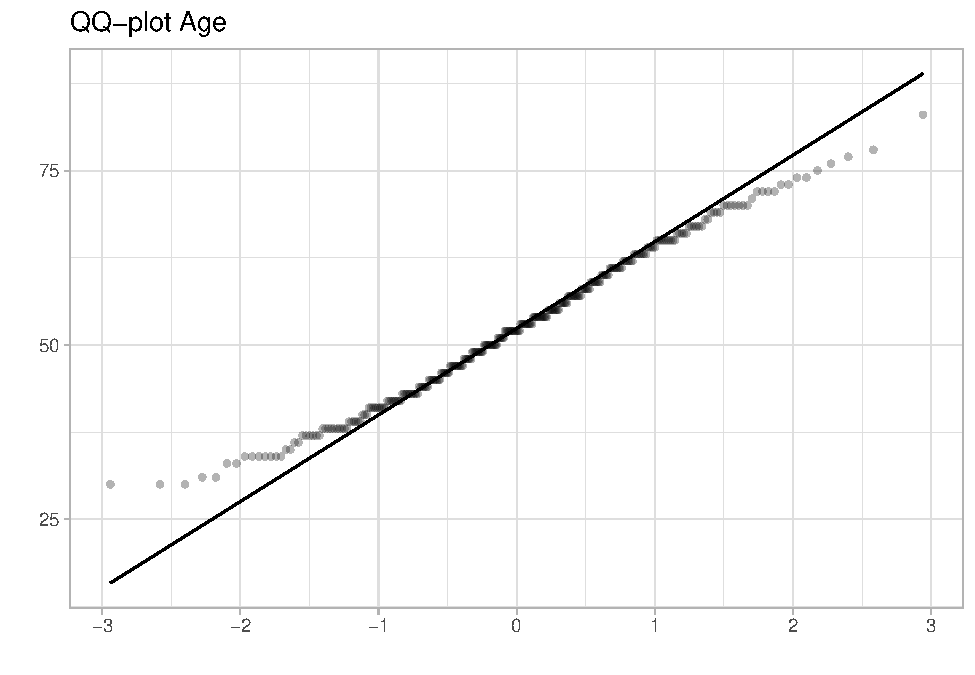
\includegraphics[width=.9\linewidth]{img/EDA2_files/figure-latex/unnamed-chunk-18-1} \caption{}\end{figure}

\begin{figure}[H]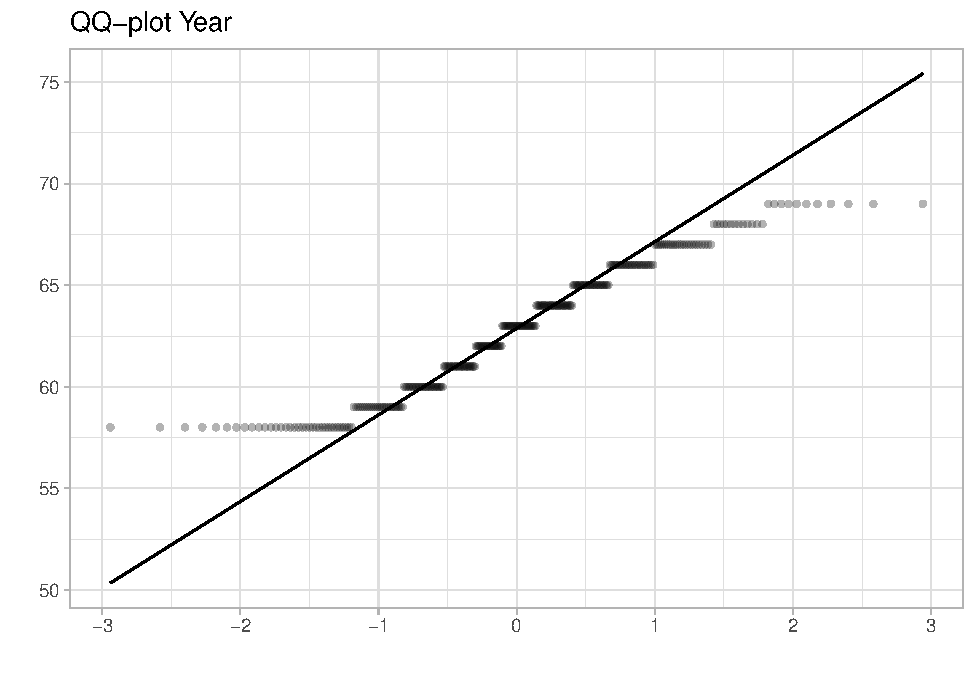
\includegraphics[width=.9\linewidth]{img/EDA2_files/figure-latex/unnamed-chunk-18-2} \caption{}\end{figure}

\begin{figure}[H]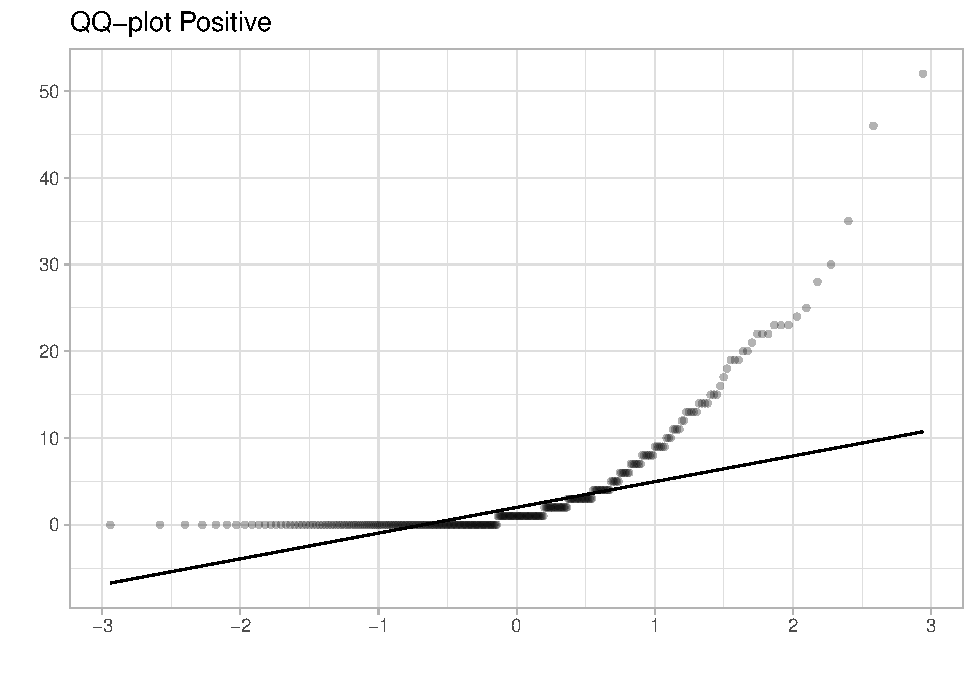
\includegraphics[width=.9\linewidth]{img/EDA2_files/figure-latex/unnamed-chunk-18-3} \caption{}\end{figure}

\begin{figure}[H]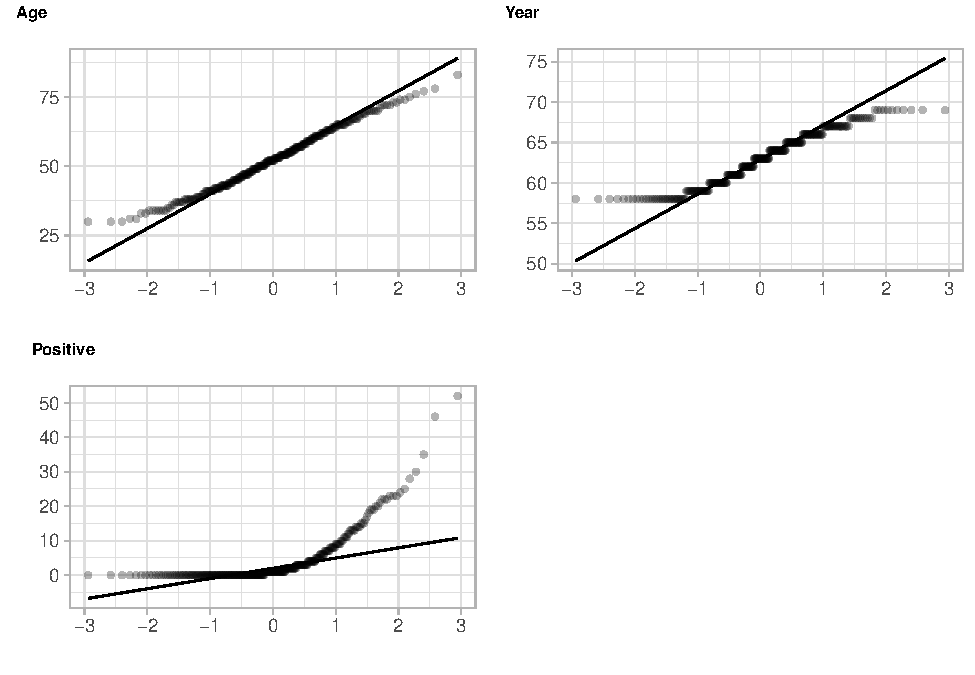
\includegraphics[width=.9\linewidth]{img/EDA2_files/figure-latex/unnamed-chunk-18-4} \caption{}\end{figure}

\newpage

La variable Positive parece seguir una distribución exponencial. Podemos hacer un plot de los supuestos cuartiles para hacernos una idea de cómo se asemeja:

\begin{figure}[H]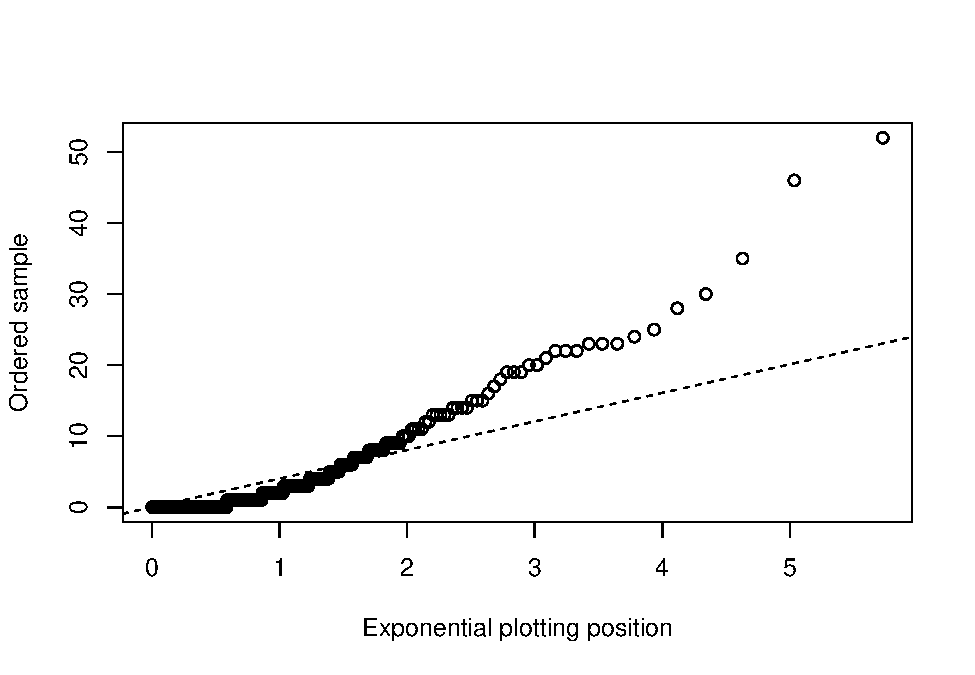
\includegraphics[width=.9\linewidth]{img/EDA2_files/figure-latex/unnamed-chunk-20-1} \caption{}\end{figure}

Ya el gráfico nos muestra que no se va a asemejar, pero podríamos verificarlo con más precisión haciendo uso de un test de Kolmogorov-Smirnov.

\paragraph{Skewness}
Claramente la única variable con skewness es Positive, con un grado positivo bastante alto:
\begin{verbatim}
Positive:  2.969176
Year:  0.07836828
Age:  0.1457859
\end{verbatim}

\subsubsection{Transformaciones}

El paquete \textit{caret} nos sugiere una estandarización a media cero y desviación típica 1. Para un problema de clasificación esto es totalmente necesario puesto que no queremos que los diferentes rangos de las variables hagan que haya información de más peso que otra.

\vspace{\baselineskip}

A excepción de KNN, los métodos de clasificación que vamos a usar necesitan la normalidad en los datos. En un caso real, si quisiéramos aplicar sí o sí esos métodos deberíamos averiguar previamente la distribución exacta que siguen esos datos para transformarla apropiadamente. 

\vspace{\baselineskip}

Por otro lado, transformaciones de Yeo-Johnson o BoxCox para reducir la skewness en Positive carece de lógica puesto que no sigue una forma normal.

\subsubsection{Anomalías}

La única variable en la que podríamos considerar anomalías es Positive. Tanto para la edad como para los años no tiene sentido, además de que hemos visto en los boxplots que en ellas todos los valores caen en el 95\% de la distribución.

\vspace{\baselineskip}

A la hora de considerar los outliers en Positive, tal y como habíamos mencionado en la descripción del problema, debemos recordar que un alto número de nodos detectados complica la operación y el pronóstico para el paciente.

Contrariamente a esta idea, podemos ver que para aquellas instancias con un gran número de positivos la cantidad de sobrevivientes en nuestro dataset está equilibrada:

\begin{verbatim}
 No Yes 
 17  23 
\end{verbatim}

Viendo que la distribución está equilibrada en estos posibles valores anómalos y tampoco tenemos conocimiento suficiente sobre el problema para considerar cuándo un número de positivos es demasiado alto, proseguimos manteniéndolos en nuestro dataset.

\subsubsection{Análisis de correlación}

Como este es un problema de clasificación, necesitamos eliminar aquellas variables correladas para que la información se aporte de manera equitativa. Las gráficas no nos han dado ninguna señal de una posible correlación, pero debemos asegurarnos de forma estadística.

\vspace{\baselineskip}

Tenemos que tener en cuenta que las variables no siguen distribuciones normales. Aunque el coeficiente de Pearson no asume normalidad (si asume varianza y covarianza finitas), podemos usar el coeficiente de Kendall para los cálculos. Independientemente del método usado vamos a obtener las mismas correlaciones en este dataset, solo varía la fuerza con la que se dan.

\newpage

\begin{figure}[H]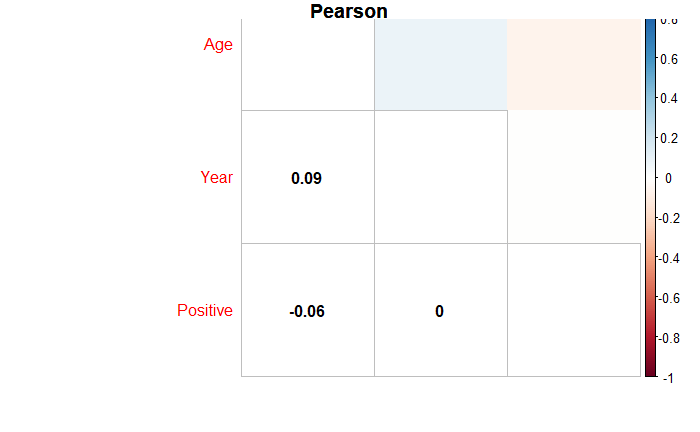
\includegraphics[width=\linewidth]{img/EDA2_files/corr1.png} \caption{}\end{figure}

\begin{figure}[H]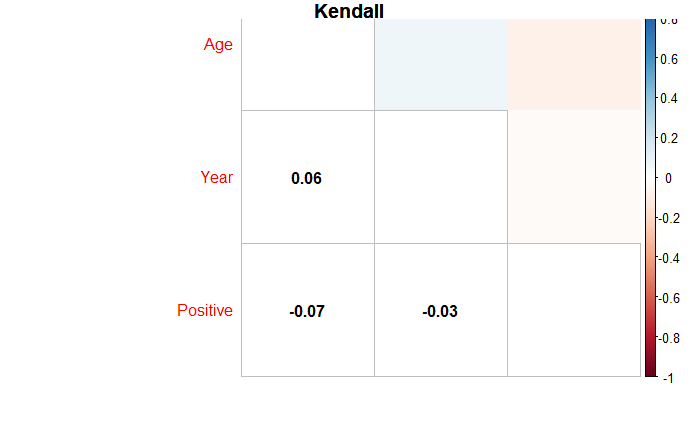
\includegraphics[width=\linewidth]{img/EDA2_files/corr2.png} \caption{}\end{figure}

\newpage

Las matrices de correlación nos muestran que no existe correlación alguna entre las variables, y un con un conjunto de scatterplot lo podemos ver gráficamente:

\begin{figure}[H]\center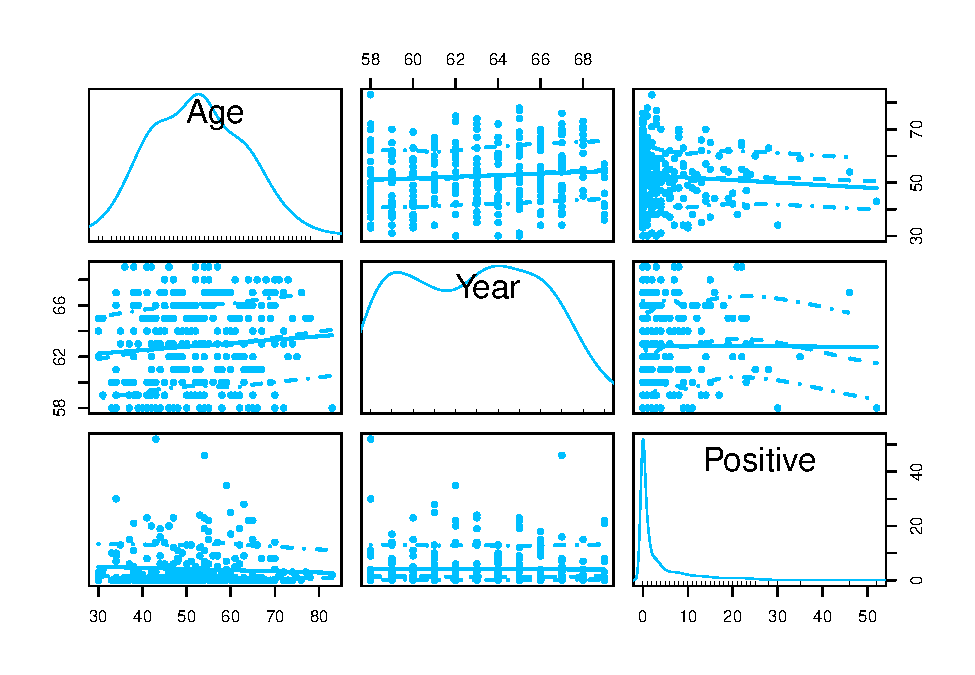
\includegraphics[width=.88\linewidth]{img/EDA2_files/figure-latex/unnamed-chunk-28-1} \caption{}\end{figure}


Adicionalmente, mostramos la distribución de las variables con su clasificación:

\begin{figure}[H]\center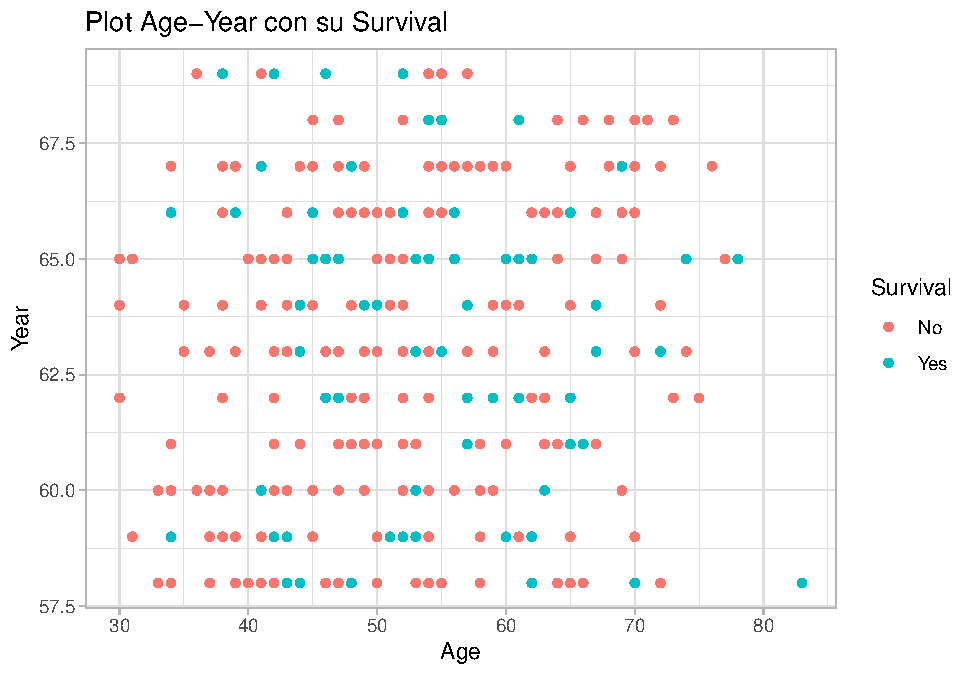
\includegraphics[width=.88\linewidth]{img/EDA2_files/figure-latex/unnamed-chunk-29-1} \caption{}\end{figure}

\begin{figure}[H]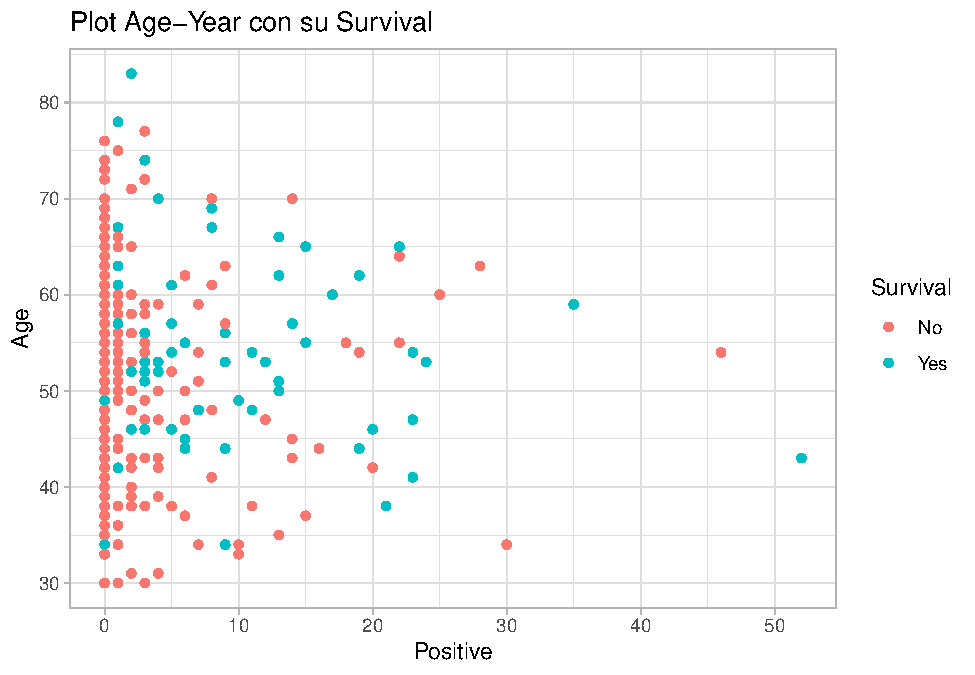
\includegraphics[width=.9\linewidth]{img/EDA2_files/figure-latex/unnamed-chunk-29-2} \caption{}\end{figure}

\begin{figure}[H]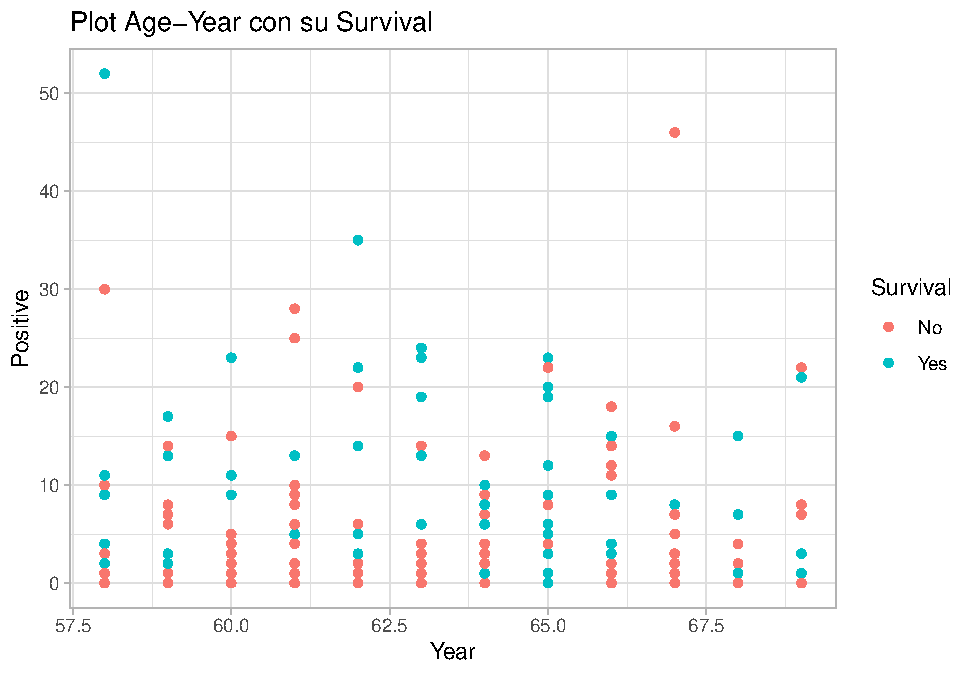
\includegraphics[width=.9\linewidth]{img/EDA2_files/figure-latex/unnamed-chunk-29-3} \caption{}\end{figure}

No se aprecia ninguna relación visual que nos ayude a clasificar el Survival.

\newpage

\subsubsection{Tratamiento de variables y ordenaciones}

Volvemos a mostrar la cabecera de los datos:

\vspace{\baselineskip}

\begin{tabular}{r|r|r}
\hline
Age & Year & Positive\\
\hline
38 & 59 & 2\\
\hline
39 & 63 & 4\\
\hline
49 & 62 & 1\\
\hline
53 & 60 & 2\\
\hline
47 & 68 & 4\\
\hline
56 & 67 & 0\\
\hline
\end{tabular}

\vspace{\baselineskip}

Para este dataset contamos con tres clasificadores con información de distinto tipo y bien organizada, por lo que no necesitamos hacer ningún tipo de ordenación/tratamiento. No existe ninguna relación entre variables sobre la información que codifican (en el sentido de que
podrían agruparse).

La variable Year solo indica las dos últimas cifras del año de operación, pero como todas las instancias son del mismo siglo nos resulta más conveniente tenerla así.

\vspace{\baselineskip}

Sobre esta variable, existe la posibilidad de hacer una discretización en intervalos, lo cuál podría ayudarnos en la clasificación. Pero observando las gráficas, vemos que no parece haber ningún agrupamiento o tendencia entre las edades y las etiquetas.
Por tanto, antes de hacer esto se debería consultar con el experto, por si hubiera un significado especial al agruparlas, y puesto que no tenemos conocimiento suficiente sobre la materia como para deducirlo nosotros, se mantienen como están.

\newpage

\subsubsection{Resolución de hipótesis}

Nos habíamos planteado las siguientes hipótesis

\begin{itemize}
    \item \textbf{H.1}: Habrá menor ratio de supervivencia cuanto mayor sea el número de nodos positivos encontrados.
\end{itemize}

\begin{figure}[H]\center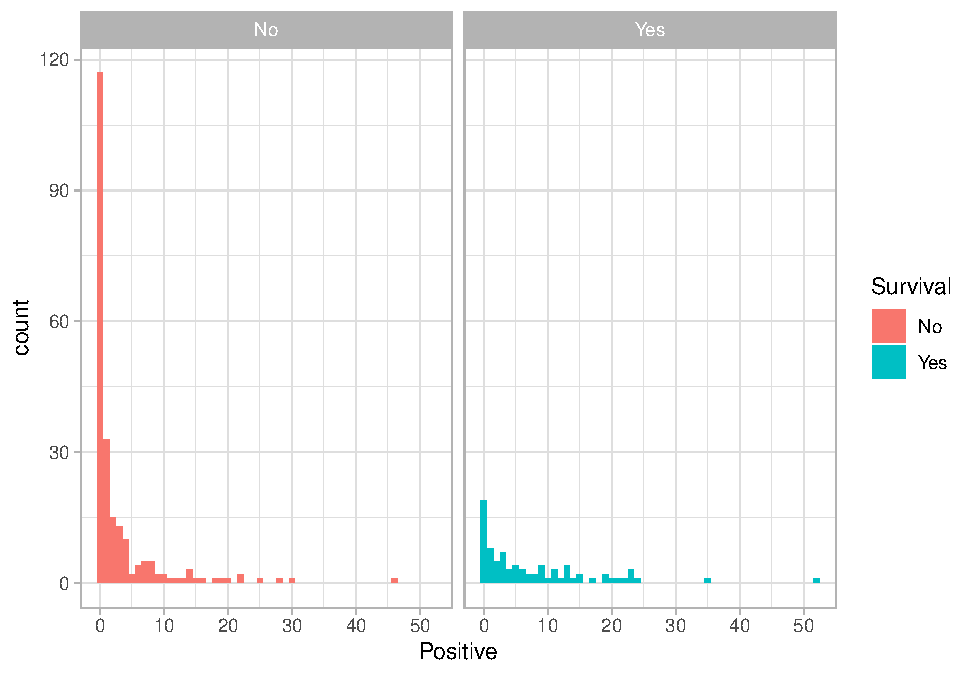
\includegraphics[width=.95\linewidth]{img/EDA2_files/figure-latex/unnamed-chunk-31-1} \caption{}\end{figure}

\begin{verbatim}
 No Yes 
 17  23 
\end{verbatim}

Vemos que la hipótesis no es cierta. Creemos que se debe a que el número de nodos no es el clasificador más importante.

\newpage

\begin{itemize}
    \item \textbf{H.2}: Habrá mayor ratio de supervivencia cuanto más joven sea el paciente.
\end{itemize}

\begin{figure}[H]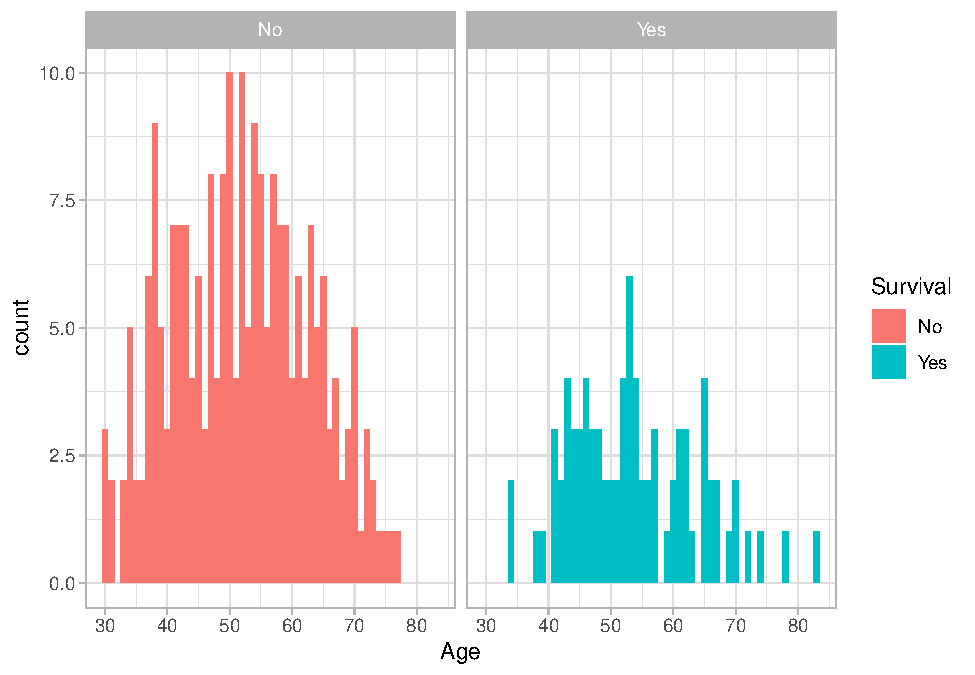
\includegraphics[width=.9\linewidth]{img/EDA2_files/figure-latex/unnamed-chunk-33-1} \caption{}\end{figure}

Si miramos los pacientes con edades \textless40 nos sale todo lo contrario:

\begin{verbatim}
 No Yes 
 36   4 
\end{verbatim}

\newpage

\begin{itemize}
    \item \textbf{H.3}: El rango de Year es pequeño. La influencia de esta variable creemos que podría darse solo si durante ese período se hubieran descubierto técnicas mejores de cirugía. Este razonamiento va orientado de cara a la población y no a la muestra. Puesto que contamos con datos de un solo hospital durante pocos años, es posible que el equipo de cirugía hubiera sido el mismo para la mayoría de pacientes.
\end{itemize}

\begin{figure}[H]\center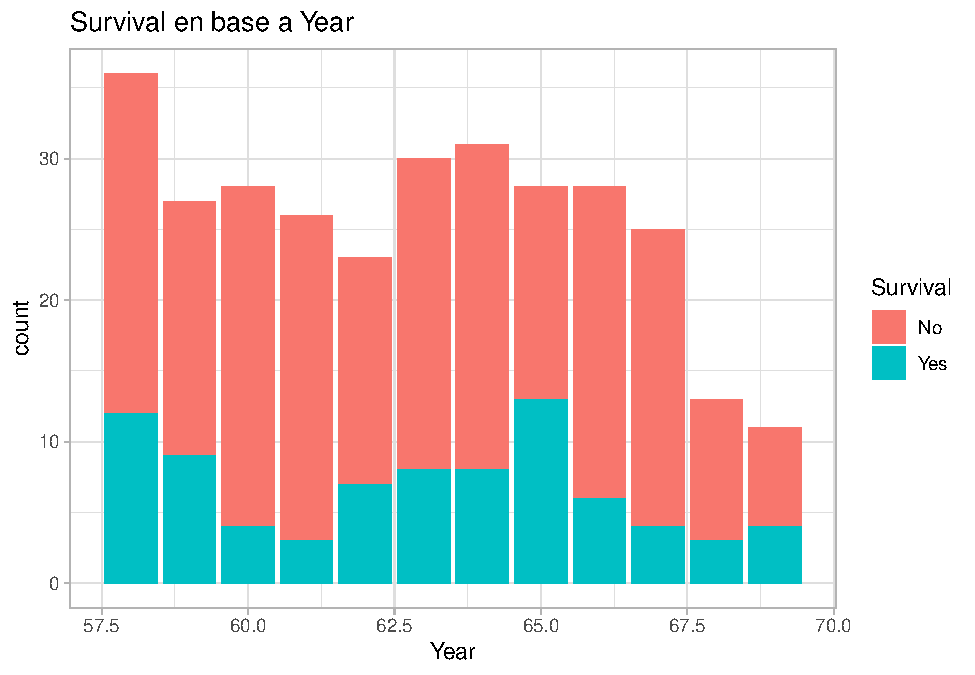
\includegraphics[width=.78\linewidth]{img/EDA2_files/figure-latex/unnamed-chunk-35-1} \caption{}\end{figure}

Decrementa el número de datos en años superiores, aunque la proporción es bastante similar con los datos que tenemos, por lo que no podemos confirmar la hipótesis:

\begin{figure}[H]\center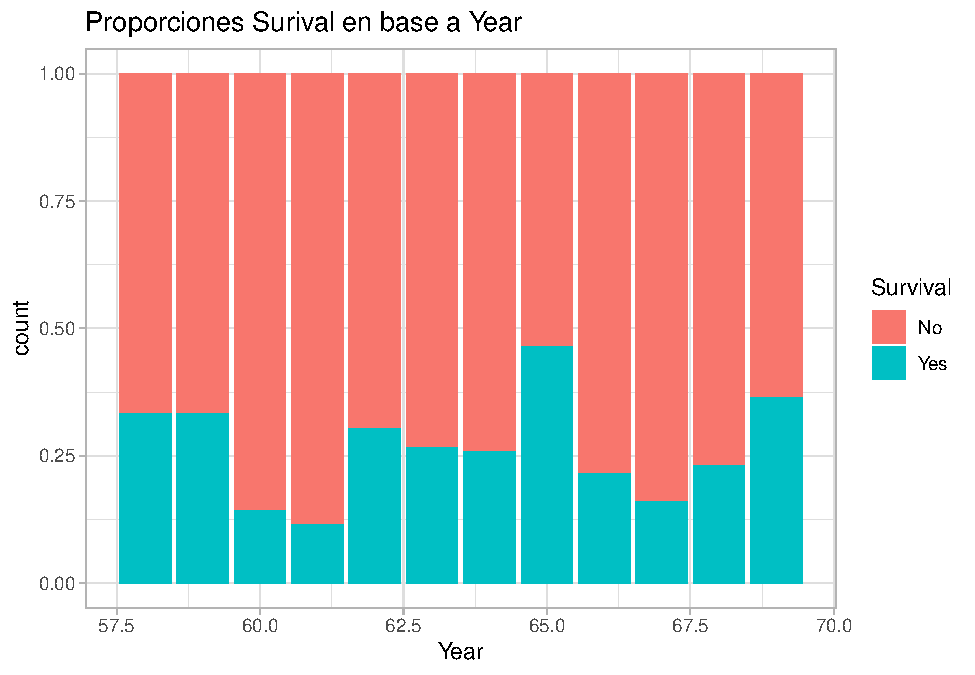
\includegraphics[width=.78\linewidth]{img/EDA2_files/figure-latex/unnamed-chunk-36-1} \caption{}\end{figure}

\newpage

\begin{itemize}
\item \textbf{H.4}: Podría haber relación entre la edad y el número de positivos,
posiblemente indicando lo tardío que se descubre el cáncer.
\end{itemize}

Un scatterplot no nos muestra visualmente ninguna aparente relación, y el análisis de correlación no nos había indicado nada:

\begin{figure}[H]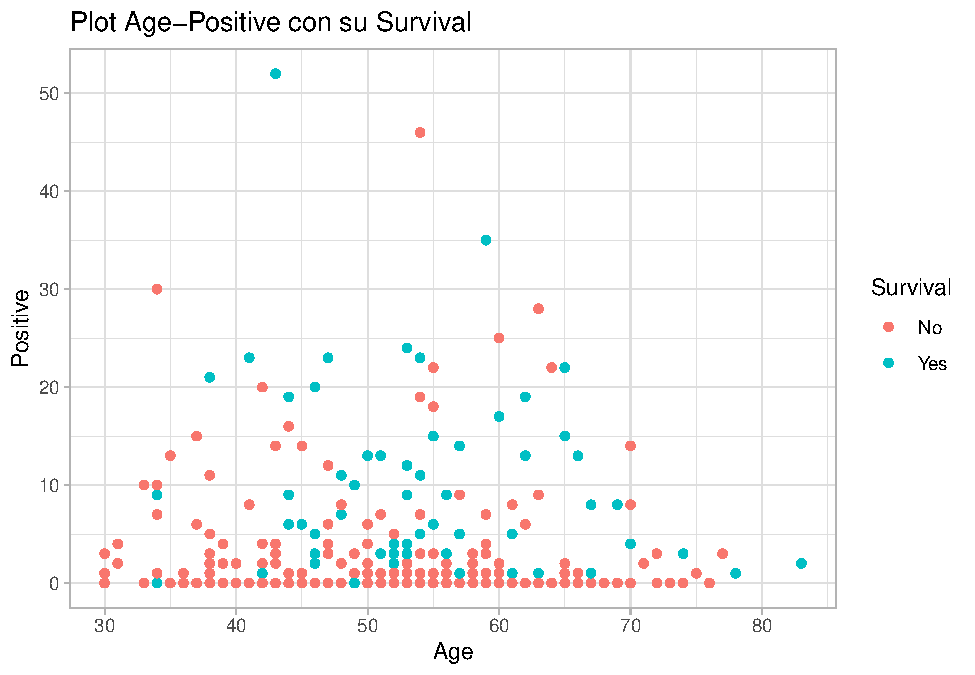
\includegraphics[width=.9\linewidth]{img/EDA2_files/figure-latex/unnamed-chunk-37-1} \caption{}\end{figure}

\subsection{Conclusiones}

Para terminar, concluímos diciendo que tenemos un dataset con pocas variables, pero con ninguna correlación entre ellas, favoreciéndonos el problema de clasificación que nos atañe. 
También hemos visto ausencia de normalidad en los clasificadores que hará que no cumplamos con las asunciones de LDA.

\vspace{\baselineskip}

Además, el dataset se encuentra desbalanceado, contando con más instancias de no supervivientes (en torno al 76\% de los datos). También se aprecian algunas instancias repetidas, sobre las que en principio creemos que se debe a una casualidad debido al bajo número de variables cuyos rangos de valores son pequeños en cada una, pero carecemos de información adicional que nos corrobore la hipótesis.

Adicionalmente, se hace notar una alta cantidad de instancias con valor de Positive cero. Por la descripción de la variable creemos que es un valor correcto y no una codificación de missing value.

\vspace{\baselineskip}

El único tratamiento realizado ha sido un preprocesado aplicando una estandarización, preparando el dataset a los algoritmos que se van a utilizar. Por la forma no normal de la distribución en Positive, no deberíamos aplicar algoritmos que la requieran.